%%%%%%%%%%%%%%%%%%%%%%%%%%%%%%%%%
\section{System Design}
\label{sec:dp-tpcelec-design}

%\fixme{separate CRO and LRO} THERE IS STRONG COUPLING BECAUSE THE LRO INHERITS THE DESIGN FROM CRO. IT IS NOT EVIDENT HOW TO DO THIS IN CLEAR CUT WAY

The \dword{cro} \dword{fe} analog electronics is based on a cryogenic \dword{asic} chip with a large dynamic range (up to \SI{1200}{\femto\coulomb}) to accomodate the charge amplification in the %\dual 
\dword{crp}. The \dword{fe} cards read \num{64} \dword{crp} channels each. They are mounted in dedicated  \dwords{sftchimney} and are located within a short distance (\SI{<1}{\metre}) from each \dword{crp} to minimize the noise caused by long cables (large cable capacitance). The cards remain accessible throughout the \dword{dpmod} operation. Each \dword{sftchimney} %hosts 
accommodates \num{10} \dword{fe} analog cards, which corresponds to the readout of \num{640} \dword{crp} channels per chimney. There are, therefore, \num{240} \dwords{sftchimney} to be installed for the charge readout in a given \dword{dpmod}.   

The differential analog signals from the analog \dword{fe} cards, carried by the twisted-pair ribbon cables and routed via an interface flange of the \dwords{sftchimney}, are digitized by the \dword{amc} cards located %in the warm conditions 
outside of the cryostat. These cards are %hosted 
installed in \dword{utca} crates placed in the immediate vicinity of the \dwords{sftchimney} (one crate per chimney). %In the baseline version of the design currently used for \dword{pddp}, each \dword{amc} digitizes \num{64} channels corresponding to reading one \dword{fe} analog card. Each \dword{utca} in such case contains \num{10} \dwords{amc} reading a total of \num{640} channels. However, an implementation with \dwords{amc} supporting a higher channel density is also being investigated for cost reduction purposes.
In the design for \dword{pddp}, each \dword{amc} digitizes \num{64} channels, corresponding to reading one \dword{fe} analog card. Each \dword{utca}  contains \num{10} \dwords{amc} reading a total of \num{640} channels. However, an implementation with \dwords{amc} supporting a higher channel density is being investigated for cost-reduction purposes. 
%\fixme{I need a picture showing the AMC, the \dword{fc} card, and the \dword{utca}!} ALL THESE PICTURES ARE PROVIDED LATTER WHEN THE RESPECTIVE UNIT IS DESCRIBED

The \dword{lro} \dword{fe} analog and digital electronics is based on a custom-built \dword{amc}. The card contains a \dword{catiroc} \dword{asic} \cite{Blin:2017}, which is used to determine %precisely 
the charge and start times of signals from each individual \dword{pmt} to high precision. In addition, a \SI{14}{bit} \SI{65}{MHz} \dword{adc} digitizes the data for continuous streaming of the \dword{pmt} signals. Each card reads up to \num{16} channels. A potential %future 
upgrade is to increase the channel density per card to \num{32} channels. The \dword{lro} cards are housed in five dedicated \dword{utca} crates located close to the \dword{pmt} instrumentation \fdth{}s.

\begin{dunefigure}[Top corner view of \dword{dpmod}]{fig:dp-tpcelec-sft-chimney-pattern}
{Corner view of \dword{dpmod} showing the pattern of the \dwords{sftchimney} and \dword{utca} crates for charge readout above \dwords{crp}.}
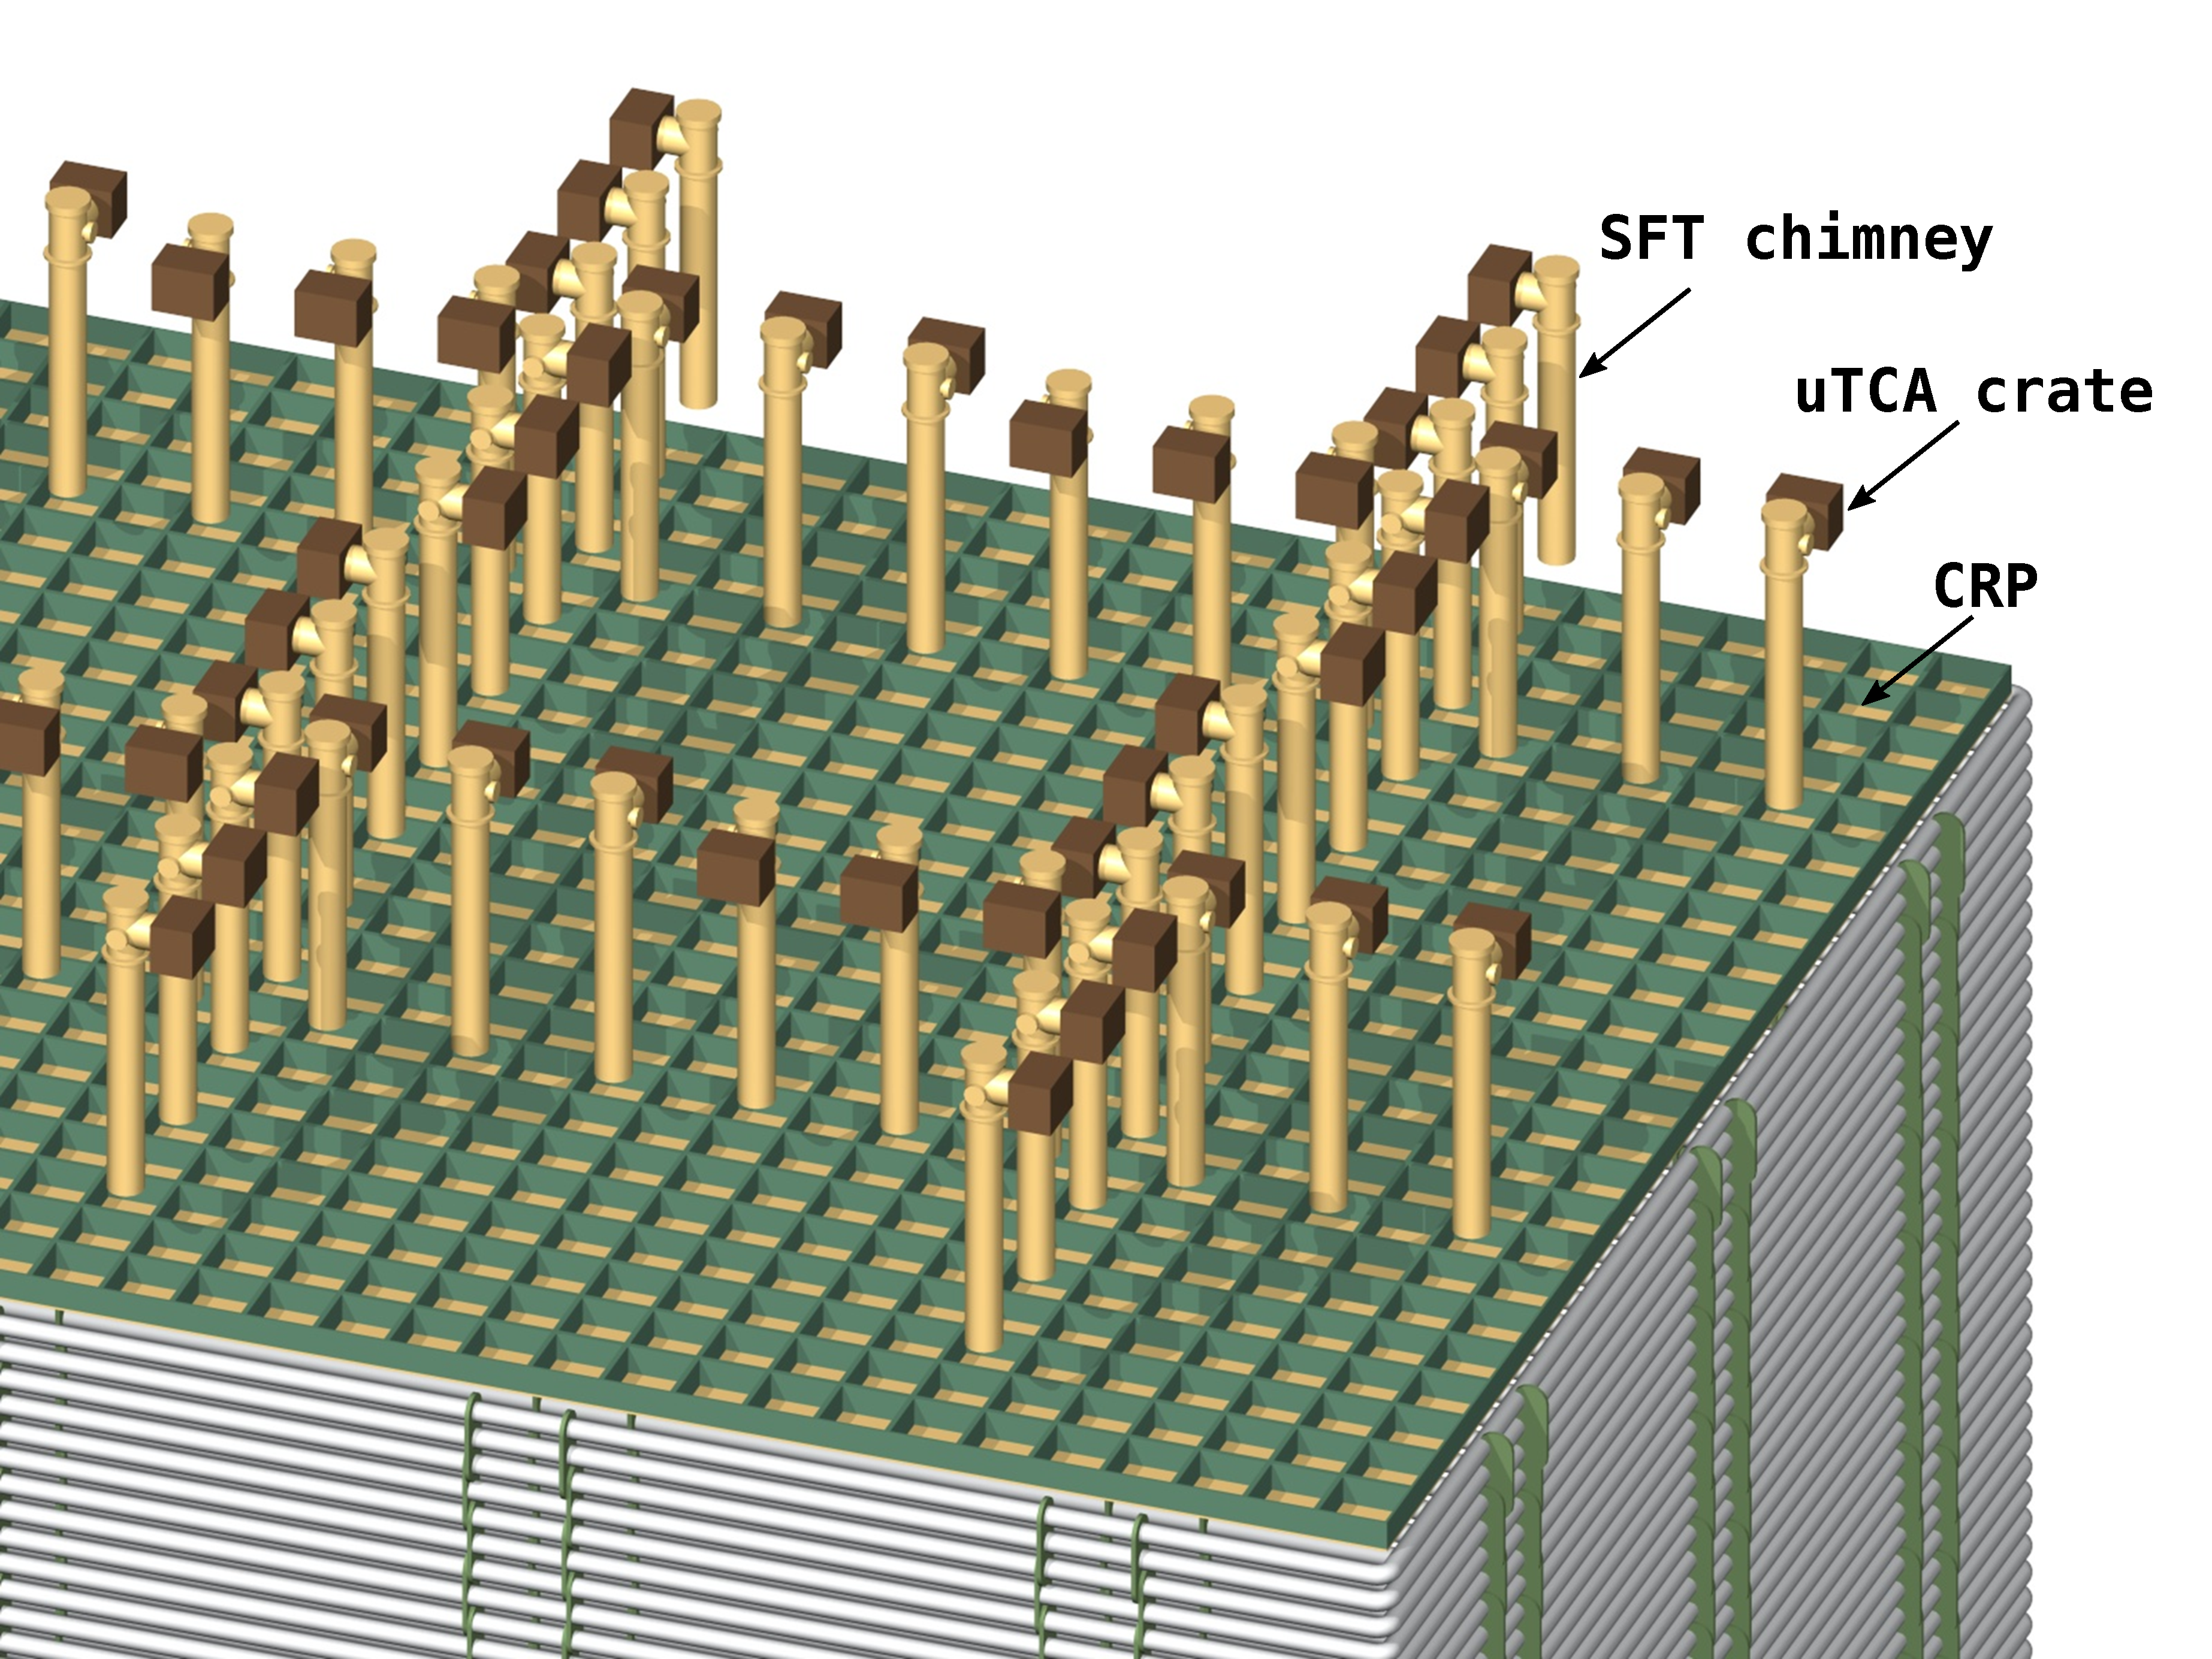
\includegraphics[width=0.6\textwidth]{dp-tpcelec-sft-chimney-pattern}
\end{dunefigure}
%\fixme{Need a similar picture for the LRO system. anne} SAME AS ABOVE

Every \dword{utca} crate contains a network switch, \dword{mch}, via which the data are sent to the  \dword{daq} and to %as well as a module 
a (\dword{wrmch}) for %clock/ 
time synchronization and trigger timestamp distribution to the \dwords{amc}. Both \dword{mch} and \dword{wrmch} require one optical fiber link each. 

The \dword{mch} switch streams the data from \dwords{amc} via a dedicated optical link. Currently \dword{pddp} uses \dword{mch} operating at \SI{10}{Gbit/s}. However, a move to \SI{40}{Gbit/s} links for the \dword{dpmod} implementation is under consideration because of the technology evolution with associated cost reductions and a possible increase in the channel density of each \dword{amc}.

The \dword{wrmch} time synchronization unit is based on the \dword{wr} system, which provides hardware and protocols for the network-based sub-\si{\nano\s} synchronization between a master and different slave nodes. The connection of the \dword{wrmch} to the \dword{wr} network is done via \SI{1}{Gbit/s} synchronous Ethernet optical link. \dword{wrmch} distributes the timing information for synchronization of the \dwords{amc} via the \dword{utca} backplane. In addition, this unit can be used to transmit triggers to the digitization units within the crate. This is achieved by sending it dedicated data packets containing trigger timestamp information. 

Figure~\ref{fig:dp-tpcelec-sft-chimney-pattern} shows a corner view of the \dword{dpmod} illustrating the pattern of the \dwords{sftchimney} and the attached \dword{utca} crates above the \dwords{crp}. Each crate/\dword{sftchimney} collects signals from \SI{3}{\meter} long strips of two \SI[product-units=power]{1x3}{\meter} \dword{crp} segments. Each chimney completely %traverses 
penetrates the cryostat insulation layers (not shown in the figure). 
%A cut-out view of the chimney illustrates the location of the \dword{fe} cards and provides the overall scale of this object. 


\begin{dunetable}
[Summary of some of the principal %numbers 
parameters of the TPC electronics system.]
{lr} {tab:dp-tpcelec-numparts}
{Summary of some of the principal %numbers 
parameters  of the TPC electronics system for charge and light readout of a \dword{dpmod}.}
Name & Number  \\ \toprowrule
   \dword{cro} \dwords{sftchimney}/\dword{utca} crates              &  \num{240}   \\ \colhline
   \dword{cro} channels per \dword{sftchimney}/\dword{utca} crate & \num{640} \\ \colhline
   \dword{cro} cryogenic analog \dword{fe} cards per \dword{sftchimney}    &  \num{10}     \\ \colhline
%   \dword{cro} Cryogenic analog \dword{fe} cards (total)                   & \num{2400}  \\ \colhline
   \dword{cro} \dwords{amc} per \dword{utca} crate                       & \num{10}      \\ \colhline
%   Charge readout \dwords{amc} (total)                                   & \num{2400}      \\ \colhline 
   \dword{lro} \dword{fe} cards  per \dword{utca} crate & \num{9} \\ \colhline
%   Light readout \dword{fe} cards (total)           & \num{45} \\ \colhline
   \dword{lro} channels per \dword{utca} crate & \num{144} \\ \colhline
   \dword{lro} \dword{utca} crate                      & \num{5} \\ \colhline
   \dword{wrmch} per \dword{utca} crate                 & \num{1} \\ 
%   \dword{wrmch} (total)                              & \num{245} \\ \colhline
%   \dword{utca} crates (total)                         & \num{245} \\ \colhline
\end{dunetable}

A short summary of some of  the number of principal components and channel granularity in the design of the \dual electronics is provided in Table~\ref{tab:dp-tpcelec-numparts}. 

%%%%%%%%%%%%%%%%%%%%%%%%%%%%%%%%%
\subsection{Cryogenic Analog Front-end Electronics}
\label{ssec:dp-tpcelec-design-cryofe}

The cryogenic amplifier \dword{asic} is the main component of the \dword{fe} analog cards. Its design is based on the CMOS \SI{0.35}{\micro\meter} technology and is an outcome of an R\&D  activity started in 2006, which resulted in several versions of the cryogenic amplifier for both \single and \dual \dword{lartpc} detectors. Two principal versions of \dword{asic} chips have been produced for \dual \dword{lartpc} operation. In the first version the amplifiers have a constant gain in signal inputs of \numrange{0}{1200}\,\si{\femto\coulomb} (\numrange{0}{40} \dword{mip}). In the second, the amplifiers have a higher linear gain for signals up to \SI{400}{\femto\coulomb} (roughly \num{10} \dword{mip} signals) and a logarithmic response in the \numrange{400}{1200}\,\si{\femto\coulomb} range. This double-slope behavior is obtained by using a MOSCAP capacitor in the feedback loop of the amplifier that changes its capacitance above a certain signal threshold. The aim of this solution is to optimize the resolution for few-\dword{mip} charge depositions while preserving the overall large dynamic range of the amplifier.

\begin{dunefigure}[Cryogenic \dword{fe} \dword{asic} properties]{fig:dp-tpcelec-fe-asic-prop}
{Cryogenic \dword{fe} \dword{asic} properties: amplifier response (left) and noise (right) at different temperatures measured at the output of differential buffer.}
\includegraphics[width=0.49\textwidth]{dp-tpcelec-fe-asic-gain}
\includegraphics[width=0.49\textwidth]{dp-tpcelec-fe-asic-noise}
\end{dunefigure}

%Figure~\ref{fig:dp-tpcelec-fe-asic-noise} 
The \dword{asic} version with the double-slope gain was selected for \dword{pddp} and has been adopted for the \dual TPC electronics design. The left plot in Figure~\ref{fig:dp-tpcelec-fe-asic-prop} illustrates the response of this amplifier for different values of the injected charge, while that on the right shows the measured noise in units of Equivalent Noise Charge (ENC) as a function of the detector capacitance at different temperatures. 
%\fixme{why in quotes?} REMOVED
For the \dword{crp} anode (detector) capacitance of \SI{480}{\pico\farad} per \SI{3}{\metre} strip, the expected noise is around \SI{2000}{e^{-}} at \SI{110}{\kelvin}. Each \dword{asic} contains \num{16} amplifier channels with differential line buffers and has a power consumption of \SI{11}{\milli\watt/channel}, surpassing the \SI{< 50}{\milli\watt/channel} requirement. 

\begin{dunefigure}[Image of an analog \dword{fe} card mounted on the extraction blade]{fig:dp-tpcelec-fe-card-blade-image}
{Image of an analog cryogenic \dword{fe} card mounted on the extraction blade, which is a part of the \dword{sftchimney} sub-system.}
\includegraphics[width=0.7\textwidth]{dp-tpcelec-fe-card-blade-image}
\end{dunefigure}
%\fixme{extraction blade is defined lower down; to fix} ADDED AN EXPLANATION THAT IT IS PART OF THE SFT CHIMNEY. IT IS ALSO COVERED IN THE GENERAL OVERVIEW SECTION

Each cryogenic \dword{fe} card, shown in Figure~\ref{fig:dp-tpcelec-fe-card-blade-image}, %hosts 
holds four \dword{asic} amplifier chips and a few passive discrete components. The input stage of each amplifier channel has a \SI{1}{\giga\ohm} resistor to ground followed by a \SI{2.2}{\nano\farad} decoupling capacitor; both are rated for \dword{hv} operation. The %function of the 
resistor grounds the \dword{crp} anode strips. A TVS diode\footnote{Bourns\texttrademark{} CDSOD323-T08LC TVS diode.} protects each input stage against discharges coming from the \dword{dpmod}. This component was selected after studying the performance of different devices for the electrostatic discharge protection by subjecting them systematically to discharges of a few \si{kV} with an energy similar to that of the \dwords{lem} in the \dword{crp}. The \dword{fe} cards also house the blocking capacitors for further filtering of the low-voltage power lines. These are first filtered at the power supply and transported via shielded cables.

\begin{dunefigure}[Noise measurements in the \dword{wa105} in different conditions]{fig:dp-tpcelec-311-noise}
{Noise of measurements in the \dword{wa105} in different conditions. Left: warm with the slow control cables connected to the cryostat flanges (red points) and disconnected (black points). The horizontal dashed line in this plot indicates the noise level expected for \SI{3}{\meter} strips. Right: warm (red points) and cold (black points) with the slow control cables disconnected. The channels with negative (positive) channel number correspond to the strips of \SI{3}{\meter} (\SI{1}{\meter}).}
\includegraphics[width=0.45\textwidth]{dp-tpcelec-311-noise-warm}
\includegraphics[width=0.45\textwidth]{dp-tpcelec-311-noise-warm-cold}
\end{dunefigure}

%While 
Although the \dword{fe} amplifier \dwords{asic} are in a shielded environment provided by the chimneys, which act as Faraday cages,
%\fixme{``which act as'' Faraday cages?} DONE 
interference from other equipment (via a noisy ground or ground loops) could significantly worsen the noise performance from the design target. Figure~\ref{fig:dp-tpcelec-311-noise} shows %some 
results of %the 
noise measurements performed under different conditions in the \dword{wa105}. The channels reading \SI{3}{\meter} (\SI{1}{\metre}) long strips correspond to negative (positive) channel numbering in the plots and the \num{1} \dword{adc} count is equivalent to about \num{900} electrons. The left plot of Figure~\ref{fig:dp-tpcelec-311-noise} shows the noise measurements performed at warm temperature with and without slow control cables (\dword{crp} \dword{hv}, \dword{crp} motors, level meters, temperature probes, etc.) connected. 
%\fixme{stuff in parentheses all pertain to slow controls?} YES THESE LIST EXAMPLES OF THE E\dword{lem}ENTS OF THE 311 SLOW CONTROL SYSTEM WHICH WERE NOT GROUNDED IN A CLEAN WAY
The noise is clearly affected by the grounding of the slow controls: the average value of the noise \rms is around \num{1.7} \dword{adc} with slow control cables connected, and decreases to about \num{1.5} \dword{adc} counts when they are removed. %As explained later,
%\fixme{ref section} IT IS EXPLAINED AT THE END OF THIS SECTION
The grounding scheme of the \dword{wa105} does not correspond to the one %foreseen for DUNE, 
planned for the \dword{dpmod}, where all electrical equipment is referred uniquely to the cryostat ground and is completely insulated from the external environment. 

One interesting feature, particularly visible with the cables disconnected, is %that the noise measured in \dword{wa105} is similar for the channels connected to the \SI{1}{\meter} and \SI{3}{\meter} long strips. 
the similarity of the noise measured for the channels connected to the \SI{1}{\meter} and \SI{3}{\meter} long strips in the \dword{wa105}. 
Given that the longer strips have %thrice 
three times the input capacitance of the shorter ones, the expected noise (see Figure~\ref{fig:dp-tpcelec-fe-asic-prop}) for these should be larger by about a factor of two as indicated by the dashed line in the plot. In addition, the noise on the short strips is lower than expected (\num{1.5} \dword{adc}) for the \SI{160}{pF/m} strip input capacitance (\num{1.7} \dword{adc}). The reason for this behavior %of the noise in the \dword{crp} of 
in the \dword{wa105} is still under investigation. %However, 
Measurements have already shown that the capacitance of the \dword{crp} anode strips is not purely to ground, but rather it is driven by the inter-strip couplings, which creates a more complicated electrical network. 

Figure~\ref{fig:dp-tpcelec-311-noise} (right) also shows a comparison of the noise measurements in the \dword{wa105} taken with the \dword{fe} electronics at warm (red points) and cold (black points) at around \SI{150}{\kelvin}. The slow control cables were disconnected in both cases. However, the cold measurements were performed with the recirculation pump active and the cathode \dword{hv} connected. 
%\fixme{present? means hv was connected?} DONE
The \rms noise averaged over all channels decreases by about 25\% from roughly \SI{1.5}{\dword{adc}} to \SI{1.1}{\dword{adc}} when the \dword{fe} analog cards are cold. For comparison, the expected signal for a \dword{mip} with the \dword{crp} gain of \num{20} should be around \SI{200}{\dword{adc}} counts. %\fixme{counts?} DONE

The overall grounding principle of the \dword{wa105} was based on %having 
using the cryostat as the ground reference. The low-voltage power supplies for the \dword{fe} analog electronics and the \dword{utca} crates were powered %via 
using insulating transformers to ensure that %they could see 
no other ground could interfere. %On the other hand, 
In contrast, the design of the slow control system did not include any insulation transformers. This equipment was grounded to the building electrical network, thereby creating an interference with the ground of the cryostat. Stricter treatment of the ground connections, as %foreseen 
implemented for \dword{pddp} and planned for the \dword{dpmod}, and a lower \dword{sftchimney} operating temperature of around \SI{110}{\kelvin} (from \SI{150}{\kelvin}) should help to further reduce the noise %levels 
from the levels observed in the \dword{wa105}.


%%%%%%%%%%%%%%%%%%%%%%%%%%%%%%%%%
\subsection{Signal Feedthrough Chimneys}
\label{ssec:dp-tpcelec-design-sft}

The \dwords{sftchimney} are designed to enable access to the \dword{fe} analog electronics for a potential repair or exchange while the \dword{dpmod} is filled and in operation. % (filled with the \lar). 
In addition, their metallic structure acts as a Faraday cage isolating the \dword{fe} \dwords{asic} from environmental interference.  Each \dword{sftchimney} hosts \num{10} analog cryogenic \dword{fe} cards (reading \num{640} channels in total).  %Some of the 
Details of the design are illustrated in Figure~\ref{fig:dp-tpcelec-sft-chimney-design}. 
%\fixme{diff between ``SFT chimney'' and just SFT?} FIXED, WAS MISSING CHIMNEY

\begin{dunefigure}[Details of the \dword{sftchimney} design]{fig:dp-tpcelec-sft-chimney-design}
{Details of the \dword{sft} chimney design.}
\includegraphics[width=0.8\textwidth]{dp-tpcelec-sft-chimney-design}
\end{dunefigure}

The chimneys are closed at the bottom and top with vacuum-tight \fdth flanges whose function is to dispatch the signal and slow control lines. The \fdth at the bottom, the cold (signal) \fdth, isolates (ultra-high vacuum tightness standard) the inner volume of the \dword{dpmod} from the chimney volume and interconnects the signals from the \dword{crp} to the analog \dword{fe} cards. The \fdth at the top, the warm (signal) \fdth, seals the chimney from the outside environment. It also passes the low voltage and control lines to the \dword{fe} electronics inside and brings out the differential analog signal lines from the \dword{fe} amplifiers. 

The \dword{sftchimney} volume is filled with nitrogen gas at near-atmospheric pressure. The temperature inside the chimney can be adjusted using a heat exchanger copper coil cooled with \lar. It is located at the bottom close to the cold \fdth around the \dword{fe} cards. %The functions of 
This cooling system %are to 
mitigates the heat input to the main \dword{dpmod} volume and provides an optimal (lowest noise) operating temperature for the \dword{fe} electronics of around \SI{110}{K}. A pressure release valve, indicated in Figure~\ref{fig:dp-tpcelec-sft-chimney-design}, protects the structure from an accidental overpressure in the inner volume. 

The expected heat input from a given \dword{sftchimney} is about \SI{20}{\watt}. This number includes the heat through the twisted-pair cables connected to the warm \fdth, the heat in the  \dword{sft} outer metallic tube, as well as the heat dissipation by the \dword{fe} cards. A total heat input from all \num{240} \dwords{sftchimney} is at the level of \SI{5}{\kilo\watt}. 

\begin{dunefigure}[Signal \fdth chimney cold flange]{fig:dp-tpcelec-sft-cold-pcb}
{\dword{sftchimney} cold \fdth flange with one of the \dword{fe} cards mounted.}
\includegraphics[width=0.6\textwidth]{dp-tpcelec-sft-cold-pcb}
\end{dunefigure}
%%%%%%%%%%%% anne to here 4/13
The analog \dword{fe} cards are inserted directly onto the PCB of the cold \fdth of \dword{sftchimney}
%\fixme{same as \dword{sft}?} DONE
(see Figure~\ref{fig:dp-tpcelec-sft-cold-pcb}). The other side of the PCB (facing inside the cryostat) hosts the connectors for the flat cables coming from the \dword{crp} anodes.  The \dword{fe} cards are mounted on \SI{2}{\m} long blades made from FR4 that enable the insertion and extraction of the electronics, and also support the flat cables carrying signals, low voltages, and slow control to and from the warm flange interface.  The blades slide along the rails installed inside the chimney at opposite sides; %which 
these rails guide the \dword{fe} cards to their respective connectors on the cold \fdth. 

Prior to the commissioning of a \dword{dpmod}, the chimneys are evacuated via a dedicated ISO standard KF16 port (see Figure~\ref{fig:dp-tpcelec-sft-chimney-design}) and then filled with nitrogen gas. This ensures the removal of % the 
any moisture that would otherwise condense around the \dword{fe} cards, once the \dword{dpmod} is filled with the \lar, damaging the electronics. To access the \dword{fe} cards once the \dword{dpmod} is cold, the stainless steel flange at the top of the \dword{sftchimney} (Figure~\ref{fig:dp-tpcelec-sft-chimney-design}) must be removed. This procedure requires continuous flushing of nitrogen gas at slight over-pressure (with respect to atmospheric) in order to prevent the humid air entering. % and generating condensation inside the chimney. 
Once a chimney is opened, it is possible to extract the blades with the \dword{fe} cards after unplugging the flat cables (two per card) connected on the inner side of the warm flange (Figure~\ref{fig:dp-tpcelec-sft-chimney-design}).

The procedure to access the \dword{fe} cards under cold operation was successfully tested during the operation of the \dword{wa105} detector. The %temperature at the 
top of the chimney was very close to room temperature, allowing manipulation of the cable connections on the warm \fdth flange without %any 
cryogenic gloves. The movement of the blades on the rails and the \dword{fe} card extraction and insertion did not indicate any mechanical problems %that could have been caused by 
due to the shrinking of various elements % due to the 
at lower temperatures.  The signals from the \dword{fe} cards that underwent %the extraction/insertion 
this process were also checked and %no malfunctioning channels were found.
all channels functioned properly.



%%%%%%%%%%%%%%%%%%%%%%%%%%%%%%%%%
\subsection{Digital Advanced Mezzanine Card Electronics for Charge Readout}
\label{ssec:dp-tpcelec-design-amc}
%THIS IS CHARGE READ OUT
The %function of the
 \dword{cro} \dword{amc} cards % is to 
 read and digitize the data from the \dword{fe} amplifiers and %then 
 transmit them to the \dword{daq} system. The cards also include a last stage of analog shaping before the \dword{adc} input. The analog \dwords{fe} produce differential unipolar signals defined with respect to a baseline offset. 
% This offset is removed and the signals are subtracted in the analog input stage of the digital electronics prior to the digitization. 
Prior to the digitization, this offset is removed and the signals are subtracted in the analog input stage of the digital electronics.
Each card has eight \dword{adc} chips (Analog Devices, AD9257\footnote{Analog Devices\texttrademark{}, 
 \url{http://www.analog.com/media/en/technical-documentation/data-sheets/AD9257.pdf}.}, Table~\ref{tab:dp-tpcelec-adc9257}), two dual-port memories (Integrated Device Technology IDT70T3339\footnote{Integrated Device Technology\texttrademark{} (IDT), \url{https://www.idt.com/document/dst/70t33391999-data-sheet}.}), and an \dword{fpga} 
 (Alterra\footnote{Alterra\texttrademark{}, \url{https://www.altera.com/products/fpga/cyclone-series/cyclone-v/overview.html}.} Cyclone V) on board. The \dword{fpga} provides a virtual processor (NIOS) that handles the readout and the data transmission. The choices for all of the components have been optimized with respect to the design requirements and technical criteria such as costs, chip footprint (small enough to fit on the \dword{amc}), power consumption, and ease of use (available functionality). 

\begin{dunetable}
[Main characteristics of \dword{adc} AD9257]
{lr} {tab:dp-tpcelec-adc9257}
{Main characteristics of \dword{adc} AD9257.}
Item &   \\ \toprowrule
Channels & \num{8} \\ \colhline
Sampling & up to \SI{40}{MSPS} \\ \colhline %/\SI{65}{MSPS}
Resolution & \SI{0.122}{\milli\volt} \\ \colhline
Dynamic range & \num{14} bit/ \SI{2.0}{\volt} \\ \colhline
Differential non-linearity & typical \num{\pm0.6} LSB\\ 
& with min. \num{-1.0} and max. \num{+1.7} LSB  \\ \colhline
Integral non-linearity & typical \num{\pm1.1}  LSB\\
& with min. \num{-3.1} and max. \num{+3.1} LSB  \\ 
\end{dunetable}
%\fixme{what's LSB (in table)?} STANDARD TERM FOR DIGITAL ELECOTRONICS REFERRING TO THE LEAST SIGNIFICANT BIT

\begin{dunefigure}[Block diagram of \dword{amc}]{fig:dp-tpcelec-amc-scheme}
{Block diagram of \dword{amc}.}
\includegraphics[width=0.9\textwidth]{dp-tpcelec-amc-scheme}
\end{dunefigure}
Figure~\ref{fig:dp-tpcelec-amc-scheme} shows block diagram of the \dword{amc} functionality. Each \dword{amc} generates a continuous compressed stream of \SI{2.5}{MSPS} \num{12}\,bit data per readout channel. The on-board ADCs operate at a rate of \SI{25}{\MHz} per channel. The data are down-sampled in the \dword{fpga} to \SI{2.5}{\MHz} by performing ten-sample averaging, which leads to further digital filtering of the noise. The data, consisting of only the  \num{12} most significant bits from each digitized \num{14}\,bit sample, are then compressed using an optimized version of the Huffman algorithm and organized in frames for transmission.  The frames contain the absolute timing information of the first data sample for reliability purposes. In the current design, each \dword{amc} has \num{64} channels and reads one analog \dword{fe} card.

The \dwords{amc} are housed in \dword{utca} crates and send their data via the \dword{mch} switch. The timing synchronization of \dwords{amc} is achieved via a \dword{wrmch} module (also housed in the crate) that is connected to the \dword{wr} network. In addition, a  \dword{wrmch} could also be used for triggered readout of \dwords{amc} by sending it dedicated packets containing trigger timestamp information over the \dword{wr} network.

In \dword{pddp}, \dwords{amc} are operated in the triggered mode, reading a \SI{4}{\milli\second} drift time window at a trigger rate of \SI{100}{Hz}, which is not far from %a 
continuous readout mode. The analog data are continuously digitized and buffered. It is possible to acquire a sub-sample of these data %can then be acquired 
by providing \dword{amc} with a timestamp generated by an external trigger. The timestamp defines the start time for the data sequence to be read, while the length of the sequence is determined by the size of the drift window. In \dword{pddp} this length corresponds to \num{10000} \SI{400}{\nano\second} samples per full drift window (\SI{4}{\milli\second}). 
%\fixme{not clear how the \num{10000} helps define the length; you say it's determined from the drift window size; clarify} DONE
 Triggers (beam counters, cosmic-ray counters, \dwords{pmt} detecting the UV light, and starts of beam spills) are time stamped in a dedicated \dword{wr} slave node (\dword{wr}-TSN), an FMC-DIO mezzanine mounted on \dword{wr} SPEC carrier card, which runs a custom firmware and is hosted in a computer. The \dword{wr}-TSN is connected to the \dword{wrgm} for synchronization and for transmission of the trigger information. The timestamp data produced by the \dword{wr}-TSN are sent over the \dword{wr} network as Ethernet packets with a customized protocol. 

%%%%%%%%%%%%%%%%%%%%%%%%%%%%%%%%%%%
\subsection{Electronics for Light Readout}
\label{sec:fddp-tpc-elec-design-lro}
%\fixme{section title: ``Digital'' Electronics for Light Reaout, in parallel with prev section?} THE ELECTRONICS INCLUDES CATIROC \dword{asic} WITH SOME ANALOG FUNCTIONALITY SO THE TITTLE SHOULD BE MORE GENERAL 
%
The \dword{lro} card is a \num{16} channel \dword{amc} containing one \num{16} channel \num{14} bit \SI{65}{\MHz} \dword{adc} (AD9249) and one \dword{catiroc} \dword{asic}. A block diagram of the prototype board used for \dword{pddp} is shown in Figure~\ref{fig:dp-tpcelec-lro-scheme} and a photo in Figure~\ref{fig:dp-tpcelec-lro-proto} . In this prototype a mezzanine board containing the \dword{asic} and \dword{adc} sits on a commercial mother board (Bittware S4 \dword{amc}\footnote{Bittware\texttrademark{}, Inc., \url{https://www.bittware.com/fpga/intel/boards/s4am/}.}) with a high specification \dword{fpga} (Alterra\footnote{Alterra\texttrademark{}, \url{https://www.altera.com/products/fpga/stratix-series/stratix-iv/overview.html}.} Stratix IV). In the final implementation for the \dword{dpmod}, the mezzanine is integrated with the layout of the \dword{amc} board developed for the charge readout.  
A proposed upgrade is a \num{32} channel card, %diminishing 
which would reduce the number of cards required and increase the channel density to \num{352} channels per \dword{utca} crate.

\begin{dunefigure}[Block diagram of \dword{lro}]{fig:dp-tpcelec-lro-scheme}
{Block diagram of \dword{lro} prototype.}
\includegraphics[width=0.8\textwidth]{dp-tpcelec-lro-scheme}
\end{dunefigure}

\begin{dunefigure}[Photo of prototype \dword{lro} card]{fig:dp-tpcelec-lro-proto}
{A photo of the \dword{lro} prototype.}
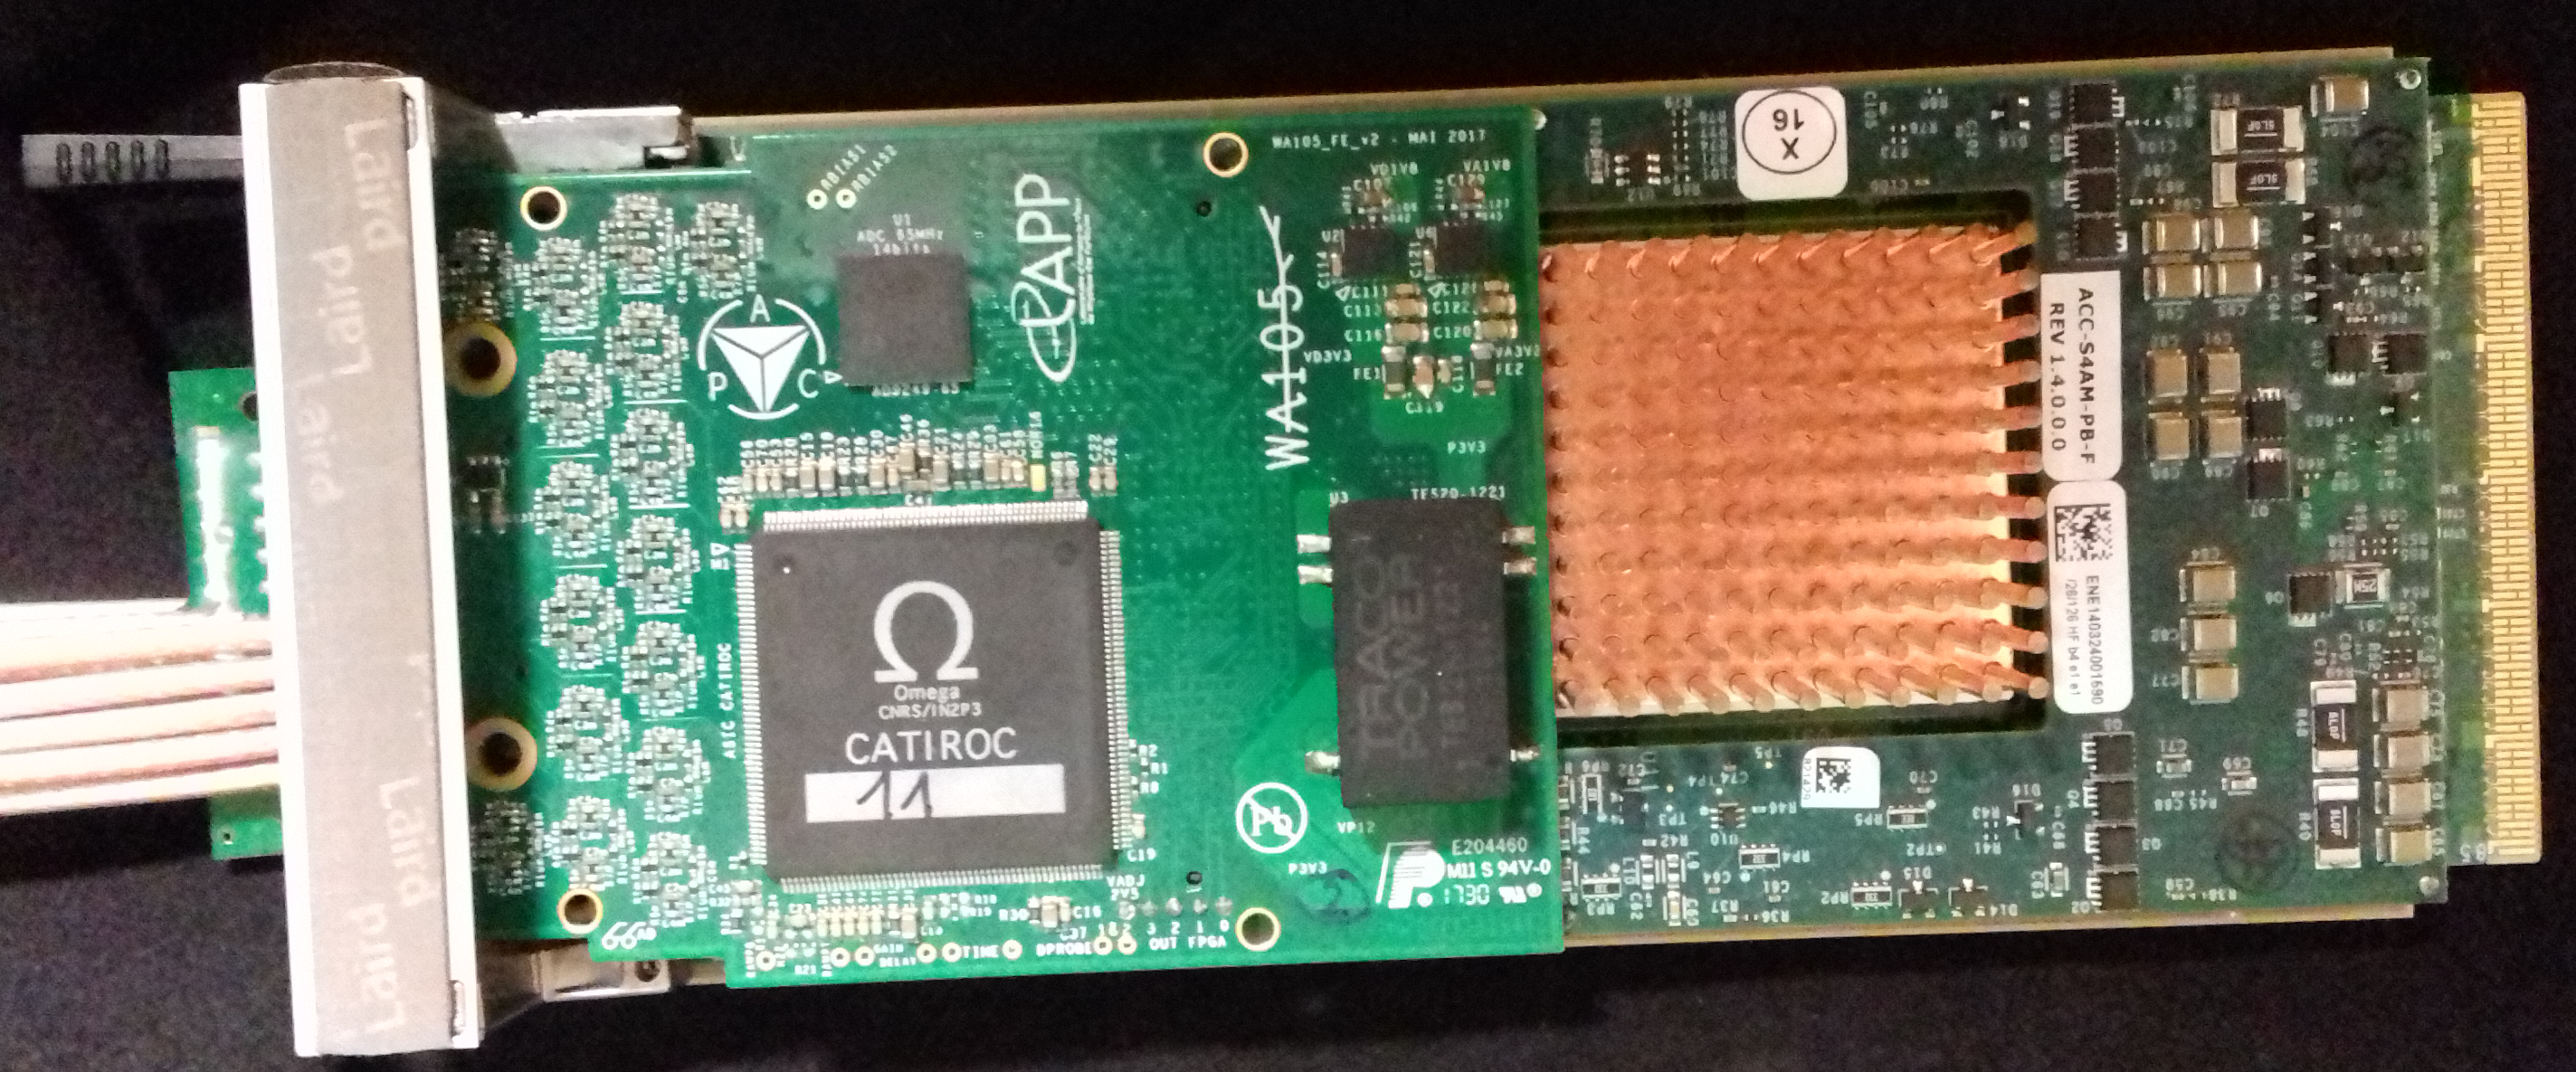
\includegraphics[width=0.7\textwidth]{dp-tpcelec-lro-proto}
\end{dunefigure}

The analog signals from each \dword{pmt} channel are split equally into two separate branches (see Figure~\ref{fig:dp-tpcelec-lro-scheme}) . One path (waveform branch), through an anti-aliasing low-pass filter and the \num{14} bit \SI{65}{\MHz} \dword{adc} (AD9249), produces continuous digitization of the \dword{pmt} waveform data, which are down-sampled to \SI{2.5}{MHz} prior to the transmission to \dword{daq}. The other (\dword{catiroc} branch) is routed directly to the \dword{catiroc} \dword{asic} for precise measurements of pulse charge and timing. Both paths produce data continuously and independently.

%%%%%%%%%%%%%%%%%%%%%
\subsubsection{Waveform branch} %\dword{adc}
%details on \dword{catiroc}
The main characteristics of the \dword{adc} used for continuous digitization of the \dword{pmt} signals are shown in Table \ref{tab:dp-tpcelec-adc9249}.
%\rms and \dword{pmt} gain?
\begin{dunetable}
[Main characteristics of \dword{adc} AD9249]
{lr} {tab:dp-tpcelec-adc9249}
{Main characteristics of \dword{adc} AD9249.}
Item &   \\ \toprowrule
Channels & \num{16} \\ \colhline
Sampling & \SI{65}{MSPS} \\ \colhline
Resolution & \SI{0.122}{\milli\volt} \\ \colhline
Dynamic range & \num{14} bit/ \SI{2}{\volt} \\ \colhline
Differential non-linearity & typical \num{\pm0.6} LSB\\
& with min. \num{-0.9} and max. \num{+1.6} LSB  \\ \colhline
Integral non-linearity & typical \num{\pm0.9}  LSB\\
& with min. \num{-3} and max. \num{+3} LSB  \\ 
%MEMORY??
\end{dunetable}
%noise llevel??

For normal operation, in the continuous mode, the digitized signals are down-sampled by the \dword{fpga} to a coarse \SI{400}{ns} sampling to match that of the \dword{cro} and limit the quantity of data streamed. 
%\fixme{is there a way to get rid of at least one or two instances of ``sample'' in the prev sentence?} DONE
The use of a higher specification \dword{adc}, with time-sampling of \SI{15.4}{ns}, allows for greater flexibility. % It is envisaged that 
For particular calibration runs, waveforms with finer time sampling could be read-out, allowing studies of, e.g., the \lar scintillation time profiles. %Even 
%During normal operation, as well, online pulse processing is possible within the \dword{fpga} using the finer time-sampled waveforms (before the down sampling), which could be used to make continuous measurements such as the rise and fall times of the pulses. 
During normal operation, as well, online pulse processing is possible within the \dword{fpga} using the finer time-sampled waveforms (before the down sampling; this would enable continuous measurements of quantities such as the rise and fall times of the pulses. Even at the coarse sampling rate of \SI{400}{ns}, studies of the \lar scintillation time profile are possible (given the long fall-time constant of $\sim$\SI{1500}{ns}) %and also 
as is matching of the electroluminescence signal (also known as proportional scintillation light) to that of the charge signal.  Low light-level signals, %such as the 
as from single or a few \phel{}s, % signals, 
will show no time structure, but will consist of one sample several LSB above the baseline. 

%%%%%%%%%%%%%%%%%%%%%
\subsubsection{CATIROC branch} %{Analog Measurements of Charge and Time}%\dword{asic}?

The \dword{catiroc} is a \num{16} channel \dword{asic} dedicated to measurement of charge and precision timing of negative-polarity \dword{pmt} signals~\cite{Blin:2017}. It auto-triggers on single \phel{}s and can sustain a high dark rate of up to \SI{20}{kHz/channel}. Charge measurements are possible over the range of \SI{160}{fC} to \SI{70}{pC} (corresponding to approximately to a range of \numrange{1}{400} \phel{}s with a \dword{pmt} gain of \num{1E6}). Timing measurements per channel can %be made with 
reflect an accuracy of \SI{200}{ps}.

\begin{dunefigure}[\dword{catiroc} \dword{asic}]{fig:dp-tpcelec-lro-catiroc}
{Functional diagram of \dword{catiroc} \dword{asic}.}
\includegraphics[width=0.8\textwidth]{dp-tpcelec-lro-catiroc}
\end{dunefigure}

Figure~\ref{fig:dp-tpcelec-lro-catiroc} shows the schematic of the \dword{catiroc} \dword{asic}. Its main properties are summarized in Table~\ref{tab:dp-tpcelec-catiroc}. The slow channel, from which precision charge and timing measurements are made, is formed by two variable-gain (\SI{8}{bit}) amplifiers followed by two variable slow shapers; one high gain for small signals, and one low gain for larger signals, and two track-and-hold stages. The slow shaper has a tunable shaping time (up to \SI{100}{ns}) and a variable gain.  If the high gain is saturated, corresponding to passing a predetermined threshold common to all \num{16} channels, the lower gain value is chosen. The chosen charge value is converted by an internal 10-bit Wilkinson \dword{adc} operating at \SI{160}{MHz}.  This slow channel operates in a ping-pong mode, with two capacitors to store the slow shaper signals, giving an effective buffer of 2 events. If both capacitors are full, a deadtime of \SI{5}{\micro\second} arises.

\begin{dunetable}
[Main characteristics of \dword{catiroc}.]
{lr} {tab:dp-tpcelec-catiroc}
{Main characteristics of \dword{catiroc}.}
Item &   \\ \toprowrule
Number of channels & \num{16}\\ \colhline
Signal polarity & negative \\ \colhline
Timing & Timestamp: 26 bit counter at \SI{40}{MHz} \\
       & Fine time: resolution $<$\SI{200}{ps}\\ \colhline
Charge Dynamic Range & \SI{160}{\femto\coulomb} to \SI{100}{\pico\coulomb}\\ \colhline
Trigger & auto-trigger \\
        & Noise = \SI{5}{fC} Minimum threshold = \SI{25}{fC} (5$\sigma$)\\ \colhline
Digital & 10-bit Wilkinson \dword{adc} at 160 MHz \\ %TWO READOUT AT 80MHZ??
        & Read-out frame of 50 bits \\ \colhline
Outputs & \num{16} trigger outputs \\
        & NOR16 \\
        & \num{16} slow shaper outputs \\
        & Charge measurement over \num{10} bits \\
        & Time measurements over \num{10} bits \\ \colhline
Main Internal &  Variable preamplifier gain \\
Programmable  &  Variable shaping and gain \\
Features & Common trigger threshold \\
         & Common gain threshold \\ 
\end{dunetable}

The fast channel is used to auto-trigger the \dword{asic} and make the fine-timing measurement. It comprises a high gain preamplifier, fast shaper (shaping time \SI{5}{ns}) and discriminator with a \num{10} bit programmable threshold that is common to all \num{16} channels. The output of the discriminator is used for the two time-to-digital convertors to get the fine timing. A coarse timestamp could also be obtained from a \num{26} bit counter running at \SI{40}{MHz}.  Only the data from the triggered channels are digitized; their information is transferred to the internal memory, which is read by the external \dword{fpga}. 

  
%%%%%%%%%%%%%%%%%%%%%%%%%%%%%%%%%
\subsection{Network-based $\mu$TCA Architecture}
\label{ssec:dp-tpcelec-design-utca}

The digital electronics is based on \dword{utca} standard which offers an industrial solution with a very compact and easily scalable architecture to handle a large number of channels at low cost.  The standard (or related standards such as \dword{atca} or xTCA) is widely used in the telecommunication industry and is being adopted by the HEP community. The backplane of the \dword{utca} crates host high-speed serial links that support a variety of transmission protocols (Ethernet, PCI Express, SRIO, etc.). In addition, dedicated lanes are available for the distribution of the clock signals to all the boards hosted in the crate.  The Ethernet-based solution has been adopted for both the data and clock distribution in this design of the \dual electronics system for both charge and light readout. 

Each \dword{amc} for either charge or light readout plugged into the \dword{utca} is connected to the crate \dword{mch} board through the backplane serial links. The \dword{mch} provides the switch functionality that enables \dwords{amc} to communicate with each other or external systems through the \dword{mch} uplink interface. In the \dual electronics system design, \dword{mch} also manages the WR clock distribution. 

\begin{dunetable}
[Bandwidth requirements per $\mu$TCA crate.]
{lr}{tab:dp-utcabandwidth}
{Bandwidth requirements per \dword{utca} crate for continuous data streaming. A compression factor of 10 for the charger readout data is assumed }   
Parameter & Value  \\ \toprowrule
  \dword{cro} data rate  &  \SI{1.8}{Gibit/s}         \\ \colhline
  \dword{lro} data rate  &  \SI{4.7}{Gibit/s}            \\ \colhline
  Current \dword{mch} bandwidth & \SI{10}{Gibit/s}              \\ \colhline
  Upgradable \dword{mch} bandwidth & \SI{40}{Gibit/s}           \\ 
\end{dunetable}

In the current design, as used for \dword{pddp}, the \dword{mch} operates with a \SI{10}{Gbit/s} uplink. Given that a \dword{utca} crate hosts \num{10} \dwords{amc} for charge readout, the required bandwidth to stream the data to \dword{daq} is about \SI{1.8}{Gbit/s}. This assumes that the data exiting the \dwords{amc} are losslessly compressed with the compression factor \num{10}. The bandwidth required per crate link for streaming the \dword{lro} data is \SI{4.7}{Gbit/s}. The \SI{10}{Gbit/s} \dword{mch} is therefore sufficient to support these data rates. However, the technology is moving towards supporting the \SI{40}{Gbit/s} rates. In addition, the channel density per \dword{amc} could also be increased for cost optimization. For these reasons an upgrade to a \SI{40}{Gbit/s} \dword{mch} could be foreseen in the future. This would also imply that the optical links connecting the \dword{daq} system to \dword{utca} \dword{mch} should be operable at \SI{40}{Gbit/s}. A summary of the required and supported bandwidths per \dword{utca} crate for continous data streaming is provided in Table~\ref{tab:dp-utcabandwidth}.

\begin{dunefigure}[Instrumented \dshort{utca} crate from the \dword{wa105}]{fig:dp-tpcelec-311-utca-image}
{Pictures of an instrumented \dword{utca} crate from the \dword{wa105}. The crate contains five \dword{amc} cards, correspondingly to the number of readout channels per the \dword{sftchimney}. The images below show the crate after the  cables are connected to the warm flange of the \dword{sftchimney}.}
\includegraphics[width=0.6\textwidth]{dp-tpcelec-311-utca-image}
\end{dunefigure}

As an illustration, Figure~\ref{fig:dp-tpcelec-311-utca-image} shows pictures of one of the instrumented \dword{utca} crates used for the charge readout of the \dword{wa105} at CERN. In this detector each \dword{sftchimney} reads \num{320} channels, thus requiring only five \dwords{amc} per the \dword{utca} crate. The two optical fiber links, one (\SI{10}{Gbit/s}) for data and the other (\SI{1}{Gbit/s}) for clock and trigger timing distribution, are visible in the images.       

%%%%%%%%%%%%%%%%%%%%%%%%%%%%%%%%%
\subsection{Timing Distribution}
\label{ssec:dp-tpcelec-wr}
% WR description and card development
The time synchronization system selected for the \dword{dpmod} utilizes a \dword{wr} network, which combines the synchronous \SI{1}{Gbit/s} Ethernet (SyncE) technology with the exchange of PTPV2 packets, to synchronize clocks of distant nodes to a common time. A high stability GPS disciplined oscillator (GPSDO) with  accuracy similar to that of an atomic clock provides a clock reference signal to be distributed over the physical layer interface of the \dword{wr} Ethernet network. The network topology is built using specially designed switches that have the standard IEEE802.1x Ethernet bridge functionality with an addition of \dword{wr}-specific extensions to preserve the clock accuracy. Time and frequency information are distributed to the nodes on the \dword{wr} network via optical fibers. The \dword{wr} protocol automatically performs dynamic self-calibrations to account for any propagation delays and keeps all connected nodes continuously synchronized to sub-ns precision. 

The sub-ns %accuracy 
precision on the clock synchronization is not strictly needed for aligning samples in the different \dword{amc} digitization units, since the %data have the timing granularity of 400 ns.
timing granularity on the data is \SI{400}{ns}. However, the \dword{wr} timing system offers readily available industrial components and the necessary protocols %needed 
for synchronization with automatic calibration of delay propagation. % and it, therefore, has been adopted. 
%This solution for the timing distribution was part of the R\&D started in 2006 and the final design for integrating this system with the readout of \dword{pddp} was completed in 2016.
R\&D on this timing distribution solution started in 2006; the final design for integrating this system, %foreseen for the \dword{dpmod}, the \dword{pddp} and the \dword{wa105} 
planned for the \dword{wa105}, \dword{pddp}, and the \dword{dpmod} readout, was completed in 2016. 
%\fixme{Is this relevant? what about timing of decision on using it for dp det module?} YES, THIS DEMONSTRATE THE STATE OF THE DESIGN READINESS

In the implementation specific to \dword{pddp}, a GPS-disciplined 
%fixme{`disciplined' seems a funny word here, but maybe that's what you call it?} YES THIS IS THE TERM USED FOR GPS TIMING SYSTEM (e.g., GPSDO)
clock unit (Meinberg LANTIME M600\footnote{Meinberg\texttrademark{}, \url{https://www.meinbergglobal.com/english/products/advanced-1u-ntp-server.htm}.}) feeds \SI{10}{MHz} and \num{1}\,PPS reference signals to a commercial \dword{wr} switch (Seven Solutions WRS v3.4\footnote{Seven Solutions\texttrademark{}, \url{http://sevensols.com/index.php/products/white-rabbit-switch/}.}). The switch acts as grandmaster of the \dword{wr} network. It is connected via \SI{1}{Gbit/s} optical links to the dedicated \dword{wr} timestamping node (\dword{wr}-TSN) and the \dword{wr} end-node slave cards present within each \dword{utca} crate (\dword{wrmch}) keeping these synchronized to its reference time. The \dword{wrgm} also communicates through a standard Ethernet port with the LANTIME unit for its date and time synchronization via NTP. The \dword{wr}-TSN module recieves analog TTL-level trigger signals, generates their timestamps, and transmits them over the \dword{wr} network to the connected \dword{wrmch} units. This timestamp information is then used by \dwords{amc} to find the data frame corresponding to the trigger. 

\begin{dunefigure}[Picture of \dword{wr} slave node card]{fig:dp-tpcelec-wrmch-image}
{Picture of the \dword{wr} slave node card (\dword{wrmch}) present in each \dword{utca} crate for time synchronization.The \dword{wr}-LEN mezzanine card is visible in the bottom right corner.}
\includegraphics[width=0.45\textwidth]{dp-tpcelec-wrmch-image}
\end{dunefigure}

The \dword{wrmch} card (Figure~\ref{fig:dp-tpcelec-wrmch-image}) enables clock/timing/trigger distribution to \dwords{amc}. It communicates with them via dedicated lines in the backplane of the \dword{utca} crate using a customized data-frame protocol. The module contains a commercial WR slave node card, the \dword{wr} Lite Embedded Node (Seven Solutions OEM WR-LEN\footnote{Seven Solutions\texttrademark{}, \url{http://sevensols.com/index.php/products/oem-wr-len/}.}), as mezzanine card. WR-LEN runs on a customized firmware which also enables it to decode the trigger timestamp data packet received over the WR network.

\begin{dunefigure}[Architecture of \dword{wr} network]{fig:dp-tpcelec-wrnet-layout}
{Architecture of WR network for time synchronization of digital readout electronics.}
\includegraphics[width=0.8\textwidth]{dp-tpcelec-wrnet-layout}
\end{dunefigure}

The architecture of the \dword{wr} network layout for one \dword{dpmod} is illustrated Figure~\ref{fig:dp-tpcelec-wrnet-layout}. It is built in a hierarchical structure from \num{16} \dword{wr} switches with \num{18} ports each,  chained with \SI{1}{Gbit/s} optical fibers. The switch at the top of the hierarchy interconnects the synchronization %grand master
\dword{wrgm} from the \dword{daq} system with the \num{15} switches in the middle layer. These are in turn connected to the \dword{wrmch} slave nodes in each \dword{utca} crate (\num{245} in total for charge and light readout). 


